%!TEX root = ../main.tex
\section{Experiment} 
\label{sec:exp}

\subsection{Experimental Settings}


\noindent \textbf{Our Experimental Scenario.} To demonstrate the performance of the \sys framework, we  analyze a simplified\footnote{why simplified?} real-world use case. The case compares  \sys framework with an open-source storage solution to build a big data processing pipeline that can facilitate business analysis. Specifically, a mobile financial application company collaborates with a mobile carrier to collect and analyze its app usage data. The company aims to understand its app usage patterns to prevent frauds and enhance its product experience. The mobile carrier provides this analytic service through an end-to-end big data processing pipeline. This pipeline includes several jobs such as data collection, normalization, labeling, and querying, as depicted in Figure~\ref{exp:fig:case}.

\noindent \underline{\textit{(a) Collection:}}  The network carrier collects mobile app data packets in  data centers across the nation via deep packet inspection (DPI) and transfers them to a centralized storage pool.

\noindent \underline{\textit{(b) Normalization:}} At the  storage pool, the data packets are normalized as records in a unified schema. Data is validated to ensure accuracy and quality. Sensitive data is shielded to protect  privacy. 

\noindent \underline{\textit{(c) Labeling:}} Labels from knowledge bases are added, so as to classify the records and identify useful insights.

\noindent \underline{\textit{(d) Query:}} After the normalization and labeling processes are completed, the  records are inserted into tables and are available for query engines. To perform analyses, the app company employs secure API calls to query the data. Figure~\ref{exp:fig:sql} illustrates an example SQL query that counts the daily active users (DAU) in different provinces. More complicated analysis, like hidden Markov and Gaussian Mixture Models\footnote{why mention models?}, can also be applied to draw user profiles and identify abnormal activities.

To support both full data and real time analyses, the network carrier builds two data flows in the pipeline. One flow processes full data in batch every two hours and the other processes stream messages constantly to deliver time-sensitive logs such as new logins, payments and password modifications. This ensures that the network carrier can effectively analyze both historical data and real-time events to make  accurate and timely decisions.

 \begin{figure}[htbp]
	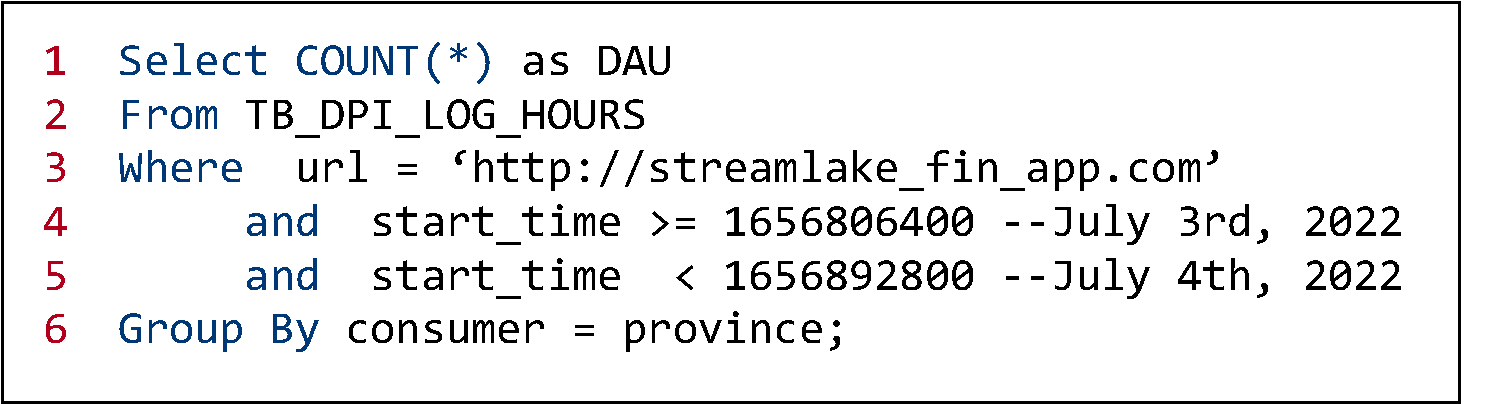
\includegraphics[scale=0.35]{figures/sql}
	\centering
	\vspace{-1em}
	\caption{Query Example of Computing DAU.}
	\label{exp:fig:sql}
\end{figure}

\noindent \textbf{Settings.} This use case is evaluated in a commodity\footnote{@} cluster using different sizes of input data packets and the results are compared with open-source storage solution Hadoop Distributed File System (\hdfs)~\cite{} and \kafka~\cite{}. The reason of why we choose the two storage systems is that in reality, China Mobile has been using them for many years, which have shown stable and good performance. Hence, it is  reasonable to directly compare with the systems that our customer (China Mobile) is using. Also, in practice, as we know, many other companies also use HDFS and Kafka to cope with similar application scenarios.
\cc{For above, do we need more justification? like why hdfs and kafka fit? or common sense?}
%These two storage systems are chosen because of their popularity in real world and are relatively easy to provide context to illustrate the usage of StreamLake.


 
  To be specific, the cluster hardware\footnote{cluster hardware?}  consists of 3 nodes, each with 24  2.30 GHz cores and 256 GB RAM. The cluster is configured as a 3-node \sys when we measure it.  While running the open-source solution, it is configured to host a 3-node \hdfs storage and a 3-node \kafka cluster simultaneously. The number of input data packets varies: 10 million, 50 million, 100 million, 500 million, and 1 billion packets. Each packet has an average size of 1.2 KB, resulting in corresponding data volumes of 12 GB, 60 GB, 120 GB, 600 GB, and 1.2 TB, respectively.

Overall, Figure~\ref{exp:fig:case} shows the data processing process.  \kafka and \hdfs serves as independent stream storage and batch storage respectively to pass data across collection, normalization, labeling and query jobs.
 As a typical ETL practice, a new copy of all data is written to \hdfs and \kafka after each job. In case it\footnote{who?} fails accidentally, a job can read its input data to reproduce the results.
 
 
 \begin{figure*}[htbp]
 	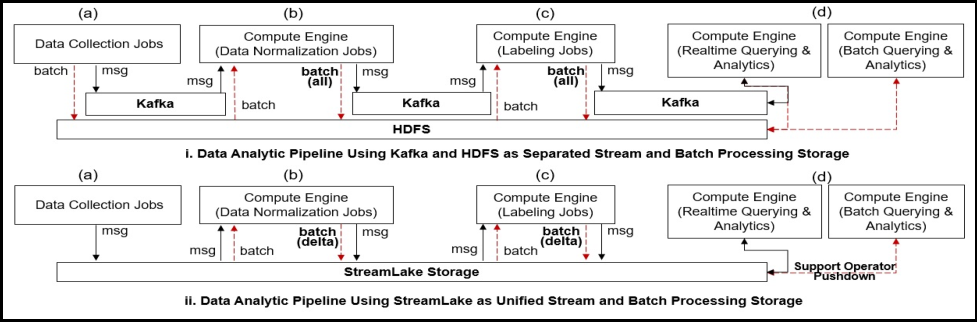
\includegraphics[scale=1.05]{figures/case}
 	\centering
 	\vspace{-1em}
 	\caption{Data Analytic Pipelines for a  Real-world Use Case.}
 	\label{exp:fig:case}
 \end{figure*}
 
  In our solution, \sys serves as a unified stream and batch processing storage. \cc{It reads messages from the data collection jobs and passes messages and aggregated batches to the same stream and batch processing engines in the normalization, labeling and query jobs.}\footnote{too many and} 
  As \sys supports time travel, only updated rows are written to the storage. When a job needs to re-run, it can use time travel to retrieve its input data.  During the query jobs, for example, the three filters in the \texttt{WHERE} clause and the \texttt{COUNT} aggregate in Figure~\ref{exp:fig:sql} are pushed down to compute in \sys, so as to  accelerate the query.


\begin{table*}[ht]
	\begin{tabular}{|c|c|c|c|c|c|c|}
		\hline
		&  \#-Data Packet & 10,000,000 & 50,000,000 & 100,000,000 & 500,000,000 & 1,000,000,000 \\ \hline
		\multirow{3}{*}{Storage Space Usage (GB)}                  & \sys              & 34         & 166        & 329         & 1,659       & 3,289         \\ \cline{2-7} 
		& \hdfs + \kafka            & 145        & 729        & 1451        & 6,901       & 13,816        \\ \cline{2-7} 
		& Ratio (HK/S)         & 4.33       & 4.38       & 4.40        & 4.16        & 4.20          \\ \hline
		\multirow{3}{*}{Stream Processing Speed (Messages/Second)} & \sys              & 301,522    & 417,303    & 518,065     & 530,077     & 546,987       \\ \cline{2-7} 
		& \kafka             & 302,611    & 413,613    & 527,826     & 531,021     & 539,893       \\ \cline{2-7} 
		& Ratio (K/S)         & 1.00       & 0.99       & 1.02        & 1.00        & 0.99          \\ \hline
		\multirow{3}{*}{Batch Processing Total Time (Second)}      & \sys             & 259        & 664        & 1173        & 4868        & 9646          \\ \cline{2-7} 
		& \hdfs              & 212        & 795        & 1548        & 7535        & 14771         \\ \cline{2-7} 
		& Ratio (H/S)         & 0.82       & 1.19       & 1.32        & 1.55        & 1.53          \\ \hline
	\end{tabular}
\caption{\sys v.s. \hdfs and \kafka.}\label{tab:case}
\end{table*}


\subsection{Overall Comparison}

Table~\ref{tab:case} shows the results. The numbers of input data packets are in the top row. The storage usage and processing time for \sys (S), \hdfs (H), \kafka (K) are in the following rows.  The ``Ratio'' represents that the ratio between \hdfs(\kafka) and \sys with respect to the storage usage or time. 
Note that HK denotes the sum of the storage usage in  \hdfs and \kafka.

The experiment demonstrates that \sys significantly improves the total storage usage and the batch processing time. The storage usage in the \hdfs and \kafka  is 4 times as much as \sys. The reason is that in \hdfs and \kafka, full data is written into the storage when each ETL job is finished, which is a common practice to support downstream jobs restart after unexpected failures. As a result, six copies of full data are written into the storage. While for our \sys, since the storage natively supports time travel, we only save one copy of full data plus updates in each ETL job, saving about 75\% storage usage.


The batch processing speed in \sys is better than \hdfs when the workload is 50 million records or more.  As the workload grows, the advantage of skipping irrelevant partitions becomes significant. \sys is 50\% faster than \hdfs when the workloads are 500 million and 1 billion records. On the other hand, \sys may not be the best choice for small workloads. When the workload is 10 million records, \sys is 20\% slower than \hdfs as it performs extra metadata management.

\cc{Why not remove the first column??}



\cc{For the above, can we correspond to the designs with respect to previous sections as the reasons of improvement}

The message stream processing speed in \sys is competitive to \kafka. \sys and \kafka process about 300 thousand messages per second when the workload is 10 million records. Both systems scale to process about 500 thousand messages per second when the workloads are 100 million and more. 


\subsection{Evaluation of Message Streaming}

To quantitively measure the message streaming service as an independent stream storage, we conduct an experiment to evaluate its throughput, latency, elasticity and volume. We select \texttt{OpenMessaging}~\cite{} as our benchmark framework as it is widely used to compare messaging platforms. A cluster with three nodes is used in this experiment for  ease of reproduction.
 To help better understand the impact of tiered storage, two sets of hardware configurations are tested. In the first set of hardware (\texttt{Set-1}), each node has 10 CPU cores, 128 GB RAM and 800 GB NVMe SSD, 3 PB SAS HDD and all the nodes are connected with 10 GB \cc{ethernet}. In the second set of hardware (\texttt{Set-2}), all the configurations are the same except that each node has additional 16 GB persistent memory to serve as an extra cache. Messages are sent from producers to consumers in a fixed size of 1 KB. The data volumes we process are 100 TB, 500 TB and 1 PB respectively. 


Figure~\ref{} shows the results. As the messages to process increase from 50000 per second to 1.5 million per second, the system throughput increases linearly, reaching a peak of 1.2 GB/s with a workload of 1.3 million message per second. \texttt{Set-1} and \texttt{Set-2} achieve almost the same throughputs, indicating that it does not improve the throughput to add persistent memory as a cache. However, as shown in Figure~\ref{}(b), persist memory reduces the latency as we expect, especially when the workload is 200k messages per second or less. Figure~\ref{}(c) shows the high elasticity of the stream storage. The service gracefully scales from 1000 to 10000 partitions in less than 10 seconds. The good scalability  demonstrates a significant advantage of the data centric and disaggregated storage design\footnote{term?}. \cc{Below is hard to follow!} Finally, Figure~\ref{}(d) compares the volumes of different storage strategies. Without scarifying the reliability, \sys provides the option to use erasure coding\footnote{term?} and column-store which can offer three to five times of volume compared to standard storage with one or more replicas. 









\subsection{Evaluation of \brain}

In this part, we evaluate the two components in \brain, $i.e.,$ auto-compaction and predicate-aware partitioning.

 
\noindent \textbf{Auto-Compaction:} To precisely evaluate the effectiveness of our automatic compaction strategy, a \texttt{TPC-H} based test bed\footnote{@ a term?} is set up to ingest data from the message streaming platform to the data lake storage, during which a compaction strategy is tested. We run the experiment with 24 GB to 90 GB data and three compaction strategies are deployed: (1) No compaction. (2) A static strategy which simply compacts data files in a 30 second interval. (3) Auto-compaction, respectively. 
During the ingestion, multiple rounds of \texttt{TPC-H} queries are executed in parallel  to obtain their end-to-end performance. As shown in Figure~\ref{}(a), the results depict how much improvement of  query performance that the compaction strategies can make, compared with baselines.
 We ca observe that the auto-compaction strategy outperforms the static one for all data volumes. As the data volume increases, the advantage becomes more significant. 
 \cc{Why?}


In addition to the query performance, we also evaluate the block utilization of the auto compaction. Specifically, we control the file ingestion speed such that we can generate different number of files to measure both the run time and the block utilization in different workloads. The run time is evaluated along with the block utilization because an ideal strategy should improve the utilization without scarifying the performance. Similar to above, we deploy three methods: (1) No compaction, (2) The static strategy compacts data files in a fixed time interval\footnote{*no need to repeat, which interval?}, and (3) Auto-compaction. We can observe that the auto-compaction outperforms the static strategy in term of block utilization. 


\cc{why?}

\cc{Ingestion speed? Below is hard to follow!}

When we deploy the auto-compaction, the system is able to identify good compaction opportunities in which there are many small files and both the file ingestion speed and the block utilization are relatively low. 

File ingestion speed is important because compaction commits will fail if there are file access conflicts. As a comparison, it is hardly to avoid unnecessary or unsuccessful compactions in the static compaction strategy hence its performance is less ideal. Figure~\ref{}(b) summarizes the results of all three test groups. Compared with no compaction and the static  strategy, our method performs better in term of both block utilization and query run time.


\noindent \textbf{Predicate-Aware Partitioning:} We also test the partitioning method on \texttt{TPC-H}  with different scale factors. We train the probabilistic model with 3\% of the data randomly sampled from the \texttt{lineitem}\footnote{@} table in a dataset generated with a scale factor of 2. After that, we obtain the optimized partitioning policy with the proposed method and evaluate our system on the full dataset with scale factors of 2, 5, 10 and 100. To evaluate the performance, we compare the resulting bytes skipped for \texttt{lineitem} table with (1) No partition (\texttt{full}). (2) Partition by the day of \texttt{l\_shipdate} (\texttt{day}).  (3) Our  method using sum-product networks (\texttt{spn}).
 We compare the results with partitioning by the day of \texttt{l\_shipdate} considering it appears frequently in the pushdown predicates. The workload includes \texttt{TPC-H} query 6, 12 and 19 which involve \texttt{lineitem} table and include predicates other than \texttt{l\_shipdate}. We skip \ other \texttt{TPC-H} queries because their performance is  mainly dominated by the joins of multiple tables, which is beyond our purpose.

The results  in Figure~\ref{}(c,d) shows that the proposed method obtains non-marginal performance gains in terms of both bytes scanned and the runtime. The fine-grained partitioning is superior on the queries in terms of data skipping compared to partitioning by the day of \texttt{l\_shipdate} because the optimized partitioning policy split the data based on other predicates except \texttt{l\_shipdate}. Even though the runtime for the queries are dominated by table joining, the optimized partitioning also demonstrated some improvements for query 6 and query 19, considering we only optimize the partition of the \texttt{lineitem} table. 


\cc{Why not reverse as previous sections?}


\subsection{Evaluation of Query Pushdown}
In this experiment we evaluate the query operator pushdown method which we believe can provide stable query runtime regardless of network conditions. This is significant in the real-world deployment as it is not always an option to upgrade the data center network. In fact, many customers who we have worked with did the opposite to ask us to reuse their existing network to reduce the overall upgrade costs. Hence, it is a critical design that the query operator pushdown method ensures the query processing time and the application service level agreements even with a constraint network bandwidth.

Two groups of clusters with different network bandwidths are used in this experiment, one with 10 Gb bandwidth and the other with 1 Gb. To precisely assess the benefits, we carefully select three live queries with data intensive operations and 4.8 TB data from a China Mobile production environment. Two different query engines, Hive and Presto, are deployed to process the SQL queries for generalization. It is observed that in the test group without query operator pushdown, the query performance varies widely across engines. When the queries are executed in the 10 Gb ethernet, Presto completes the jobs in about 900 seconds while Hive takes around 1200 seconds. When network bandwidth drops to 1 Gb, all the execution time soars to over 3000 seconds. As a comparison, we applied query operator pushdown in the second test group. The runtime of all the queries is close to 900 seconds with less than 10 difference, regardless of compute engines and network bandwidths. This means a 4 times performance advantage when the engine process queries in a 1 Gb bandwidth network. In summary, we can conclude that our generalized query operator pushdown method introduces stable and high performance to query processing in a storage-disaggregated architecture. 




\subsection{China Mobile Use Case}